\documentclass[conference]{IEEEtran}
\IEEEoverridecommandlockouts
\usepackage{cite}
\usepackage{amsmath,amssymb,amsfonts}
\usepackage{algorithmic}
\usepackage{graphicx}
\usepackage{textcomp}
\usepackage{xcolor}
\usepackage{url}
\usepackage{wrapfig}
\usepackage{float}
\usepackage{lscape}
\usepackage{longtable}
\usepackage{booktabs}
\def\BibTeX{{\rm B\kern-.05em{\sc i\kern-.025em b}\kern-.08em
    T\kern-.1667em\lower.7ex\hbox{E}\kern-.125emX}}
\begin{document}

\title{ESCAPE Y2K - An Integrated Escape Room}

\author{Kyle L. Sedgwick, Jake D. Bales, Nami Eskandarian}

\author{\IEEEauthorblockN{1\textsuperscript{st} Kyle L. Sedgwick}
    \IEEEauthorblockA{\textit{College of Engineering} \\
        \textit{University of Utah}\\
        Salt Lake City, U.S \\}
    \and
    \IEEEauthorblockN{2\textsuperscript{nd} Jake D. Bales}
    \IEEEauthorblockA{\textit{College of Engineering} \\
        \textit{University of Utah}\\
        Salt Lake City, U.S \\}
    \and
    \IEEEauthorblockN{3\textsuperscript{rd} Nami Eskandarian}
    \IEEEauthorblockA{\textit{College of Engineering} \\
        \textit{University of Utah}\\
        Salt Lake City, U.S \\}
}



\maketitle

\begin{abstract}
    “ESCAPE Y2K” is an interactive escape room experience that relies on computer
    engineering as its main control source. The escape room is built to be an autonomous,
    immersive, sci-fi, horror experience using digital/analog circuit design, image/audio
    processing, communication protocols, and embedded computing. Players
    will interact and solve puzzles under a time limit while avoiding fictional threats within
    the game in order to complete the experience and win. This is done with a time travel mechanic
    that allows players to forward or reverse an artificial clock that changes the time within
    the room and activates certain events that could both benefit and disadvantage them.
\end{abstract}

\begin{IEEEkeywords}
    Analog, Embedded Systems, Escape Room, Horror, Interactive, Networking, Science Fiction
\end{IEEEkeywords}

\section{Introduction}
Escape rooms are a fun and engaging way to promote critical thinking and puzzle solving for children and adults
alike. In most established escape rooms, there is a level of behind the scenes interaction with a room operator,
triggering events and unlocking clues as the players progress. This usually works quite well and allows for some
additional variability if the operator is given some creative freedom with how they run the escape room. However,
it also has an inherited limitation with requiring an operator for the room to function. Potential exists for an
autonomous escape room where players follow a game script without the requirement of an external human operator.
This project determines to create a system and design philosophy that allows for a more streamlined and easily modifiable
process for making more complex and dynamic escape rooms. Custom analog and digital systems, as well as a control program
executing on a central server drives the escape room's interactive elements. A solution such as this can greatly
heighten scopes and stakes of escape rooms in the future, providing uniquely exciting experiences for the players
and eases the jobs of the room owners due to automation.
\\
\indent The escape room created for this demonstration is ``Escape Y2K'', a science fiction analog horror experience. 
Inspired by the public panic caused by the Y2K scare, spurred from unknown consequences as digital system
clocks update their year count to '00' and the ambiguity between it's interpretation as '2000' (Y2K) or '1900',
``Escape Y2K'' will be set before the start of the new millennia on January 31, 1999. Due to technological disturbance,
scientists have discovered a creature that will destroy all of humanity, its presence and danger felt in televisions
spread across the room. It is up to the team of players to discover how to send this creature back using puzzle solving
and time travel. Using a remote to forward and reverse a clock that represents in-universe time, they can stop the year
from turning to 2000 which causes total system failure and humanity to end. This inspires the tagline of the game:
``Don't let the clock strike midnight.''

\section{Background}
\indent Escape rooms provide participants with an interactive and exciting puzzle experience.
Players start by being ``locked'' in a room (for safety reasons, players are never really
locked inside) with a set of instructions that lead them through a series of puzzles. Some of
these puzzles are more traditional, such as solving a cypher or figuring out a combination for a lock,
while others make the players think a little bit deeper. Many of these puzzles are on the simple size in
an attempt to have a good balance of fun and difficulty. And, many of these rooms attempt to fit their
puzzles within a certain theme, such as escaping from an Egyptian tomb or trying to escape from the zombie
apocalypse~\cite{wikipediaEscapeRoom}. In order to successfully escape, it is expected that the team of players
all work together to solve every puzzle before time runs out.
\\
\indent Instead of using a large amount of analog puzzles and a ``host'' that is in charge of controlling which parts of
the room are locked and unlocked when players complete certain actions, the room will adapt and progress on its
own as players advance through the various puzzles. A similar idea was done by the 2021 Technical Symposium with
``a course with the overarching goal of designing and constructing an automated escape room''~\cite{germanEscapeRoom}. Outside
of that however, most of the effort will be drawn from a creative process for telling a story; providing presence
to players by immersing them with puzzles using old technology. Old phones, cassette players, televisions, and other
props from the Y2K era will be modified for horror and also allow for puzzle solving. All of this will be done
with the explicit purpose of showing off the wireless communication between the server and the puzzles to keep track
of player progression. 

% ************************************************************************************************************************
% ************************************ THIS IS THE MAIN SECTION TO REVISE FOR THE FINAL REPORT ***************************
% ************************************************************************************************************************
\section{Project Implementation}
While many aspects of our escape room are likely to be somewhat modular, and able to be re-arranged quickly,
some puzzles and in-game events will demand certain elements of the room to be set up in specific locations relative
to each other. For example, the clock controls, game clock, and action clock should all be in close proximity to each
other for ease of access. The CRT TVs should be pointed across the audio cassette player to limit
access during certain events. Finally, props need to be kept in repeatable
locations or lock boxes for consistency in certain puzzles.
\\
\indent In the below diagrams, there are a few key elements to notice. The black boxes with white screens
represent the CRT TVs that have sensors and lights to trigger during in-game events. The
grey towers are filing cabinets, to play into the office aesthetic of the game. The light green slab on the
desks in the corner is where we will have the chessboard, and the yellow head represents one of the busts
that will be included in some puzzles. The center podium will hold the cassette player. Finally, the orange circle
is the time clock, and the nearby green box represents the clock controls.

\subsection{Safe-Cracking Puzzle} %Jake
One of the puzzles that we implemented was a safe cracking puzzle. A hint for this puzzle was recorded on a cassette tape
that would help the players know which numbers they needed to turn the safe to. Once the puzzle was reset by turning the dial
to zero and holding the reset button until the lights flashed, if they turned left until they got to 33, right until they got to 72,
and left again until they reached 11 then the puzzle would be solved! However, players were only able to solve this puzzle when the
player clock (the giant physical clock) displayed a time between 2:15 and 4:30. If all of the above conditions were met, a puzzle box
would open, showing them a plugboard combination.

\subsection{Potentiometer Tuning}

\subsection{Radio Number Station}

\subsection{Audio Control and Tapes}

\subsection{Props and Hints}

\subsection{Adding Time} %Jake

\subsection{TVs, State, and Detection}

\subsection{Time Control and the Clock}

\subsection{Wireless Communication and Circuit Design} %Jake

\subsection{Box Control}

\begin{figure}[ht]
    \centering
    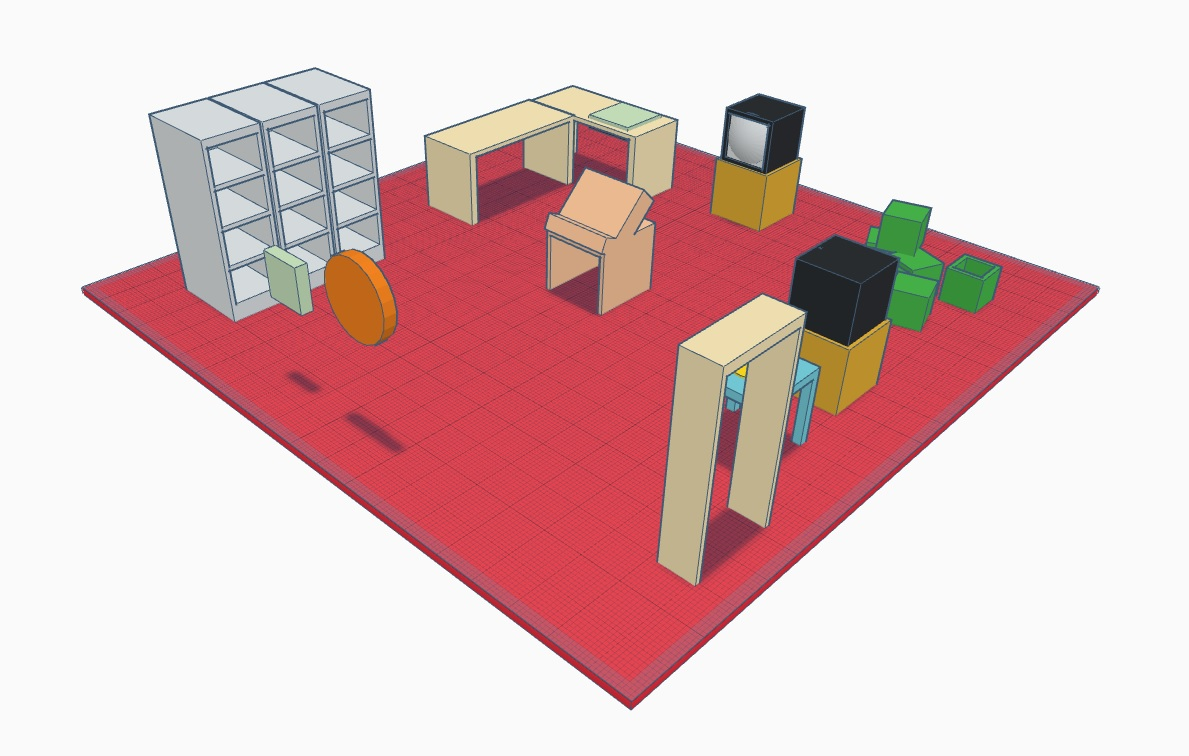
\includegraphics[width=0.90\columnwidth]{Images/EscapeRoomIsoFront.jpg}
    \caption{Front isometric scale depiction of the initial escape room layout.}
\end{figure}

\begin{figure}[ht]
    \centering
    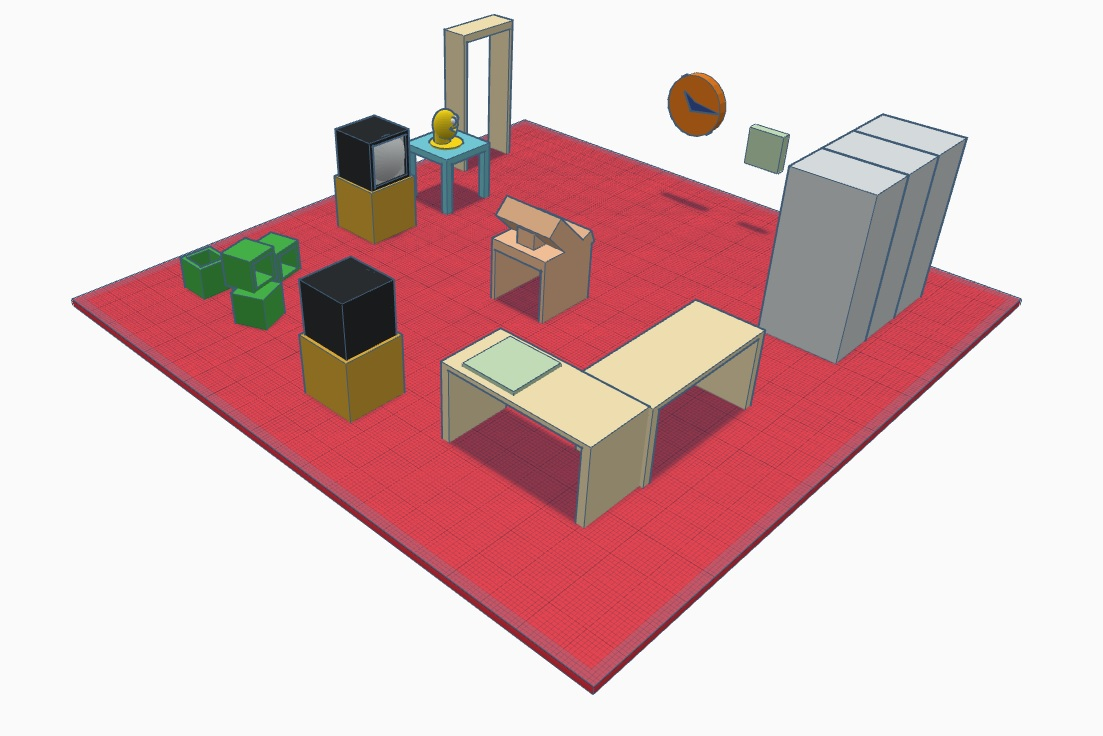
\includegraphics[width=0.75\columnwidth]{Images/EscapeRoomIsoRear.jpg}
    \caption{Rear isometric scale depiction of the initial escape room layout.}
\end{figure}


\section{Puzzles in our Escape Room}
This section contains a list of all of the puzzles that our escape room will feature, as well as
the solution to each of them. If you haven't already experienced the escape room, be warned that
this section does contain spoilers and will prevent you from experiencing the joy of solving the
puzzles on your own.
\\

% *************************************************************************************************************************************
% ************************************* THIS SECTION MUST BE REVISED ******************************************************************
% *************************************************************************************************************************************

\indent This section will be greatly expanded on as we decide what other puzzles we want to incorporate and how they will function.
A stretch goal we have is to have a pool of around 10-15 puzzles that can be randomly selected, so that each time a player is in the
room the experience will be different from the last. More may be added, depending on time contstraints and how many ideas we
have, but this is the idea for now.
\\
\indent Furthermore, we want to develop puzzles that take between 3-5 minutes to solve. This will be a hard balance
to achieve because we really want the puzzles to feel rewarding to solve, but also not frustrate the players
to a point when they are no longer able to continue with the escape room. Various tests will be run on friends, family members,
and anyone else who would like to help us tune the puzzles until they arrive at a happy medium.


\subsection{Bust} %Nami we gotta change this one cuz it talks about the chess piece
A small bust of a statue's head will be attached on a disc and situated
on a podium. This bust can be rotated physically, which will rotate the
disc under it as well. On the podium is a small hole that may contain a key
or chess piece. The disc will also have an indent on it. When the players
rotate the bust, if the disc is rotated so that the indent is overlapping
with the hole on the podium, the players are able to retrieve the key
or chess piece. As a bonus, the direction the bust is facing will be either
the lock the key unlocks or a clue as to where the chess piece goes.

\subsection{Tape Player}
An audio cassette player will be centered in the room, with one tape nearby
to be played as players first enter the room. The general function of the tape
player will be to both give the players story elements and instructions on
puzzles as they play, as well as be used to play clues or hints to the active
puzzle that the players are working on. Beyond these basic functions of the
cassette player, we will run wires from our microcontroller and digital audio
player into the built-in speaker of the cassette player to inject noises or music
files while the cassette player is not actively in use, or no tape is even in the
deck. This will add to the horror experience, and emulate rouge transmissions
being received over the duration of the escape experience.

\subsection{Encoded Audio/Radio Signal}
%KYLE, DONT FORGET TO TALK ABOUT YOUR SUPER DOPE ANALOG WAVE PUZZLE IDEA WITH PLAYING THE RIGHT CASSETTE TAPE
There are many devices available to convert an audio signal, supplied via an AUX audio cable
to a radio signal that can be transmitted via bluetooth or a similar radio protocol. One interesting
application of this intended to be implemented in this project is to either have a personal voice recorder
or audio cassette have a ``key'' encoded in the audio that will need to be transmitted to another
device in the room to unlock a lock box or clue. For example, a voice recorder may be found which has
a password spoken by a specific person's voice as a room access key. This recording will be played
to the correct access point to complete the puzzle and unlock the next item.

\subsection{All other puzzles...}
Currently, we have this limited number of planned puzzles, but more puzzles are expected to be added
as stretch goals. We plan on having this escape room experience last only between 20 to 30 minutes,
but this is a flexable duration that may change if time permits us to add a system that selects
only certain puzzles to be used in a given playthrough. This would allow for greater variability,
and for users to play the escape room more than once and solve different puzzles each time.
Once we have more base systems in place to make puzzles designing to be more streamlined, we can add
both to the number and complexity of puzzles.

\subsection*{Clock}
The clock that we have planned to use will be controlled through a single motor that turns the
dial used to set the clock (if you were planning on using it normally). We have already created
a mechanism that will control the clock and also allow others to control the clock as well. Under
no user input, the clock will function as normal, ticking forward at a constant rate of one hour per
minute. There are also two buttons, a fast-forward and a reverse button, that give players control
over the time that the clock is displaying. Once a button is pressed, a motor spins the clock
either forward or backwards, adjusting the events that are taking place in the room. An image of
the clock has been included below.

\begin{figure}[ht]
    \centering
    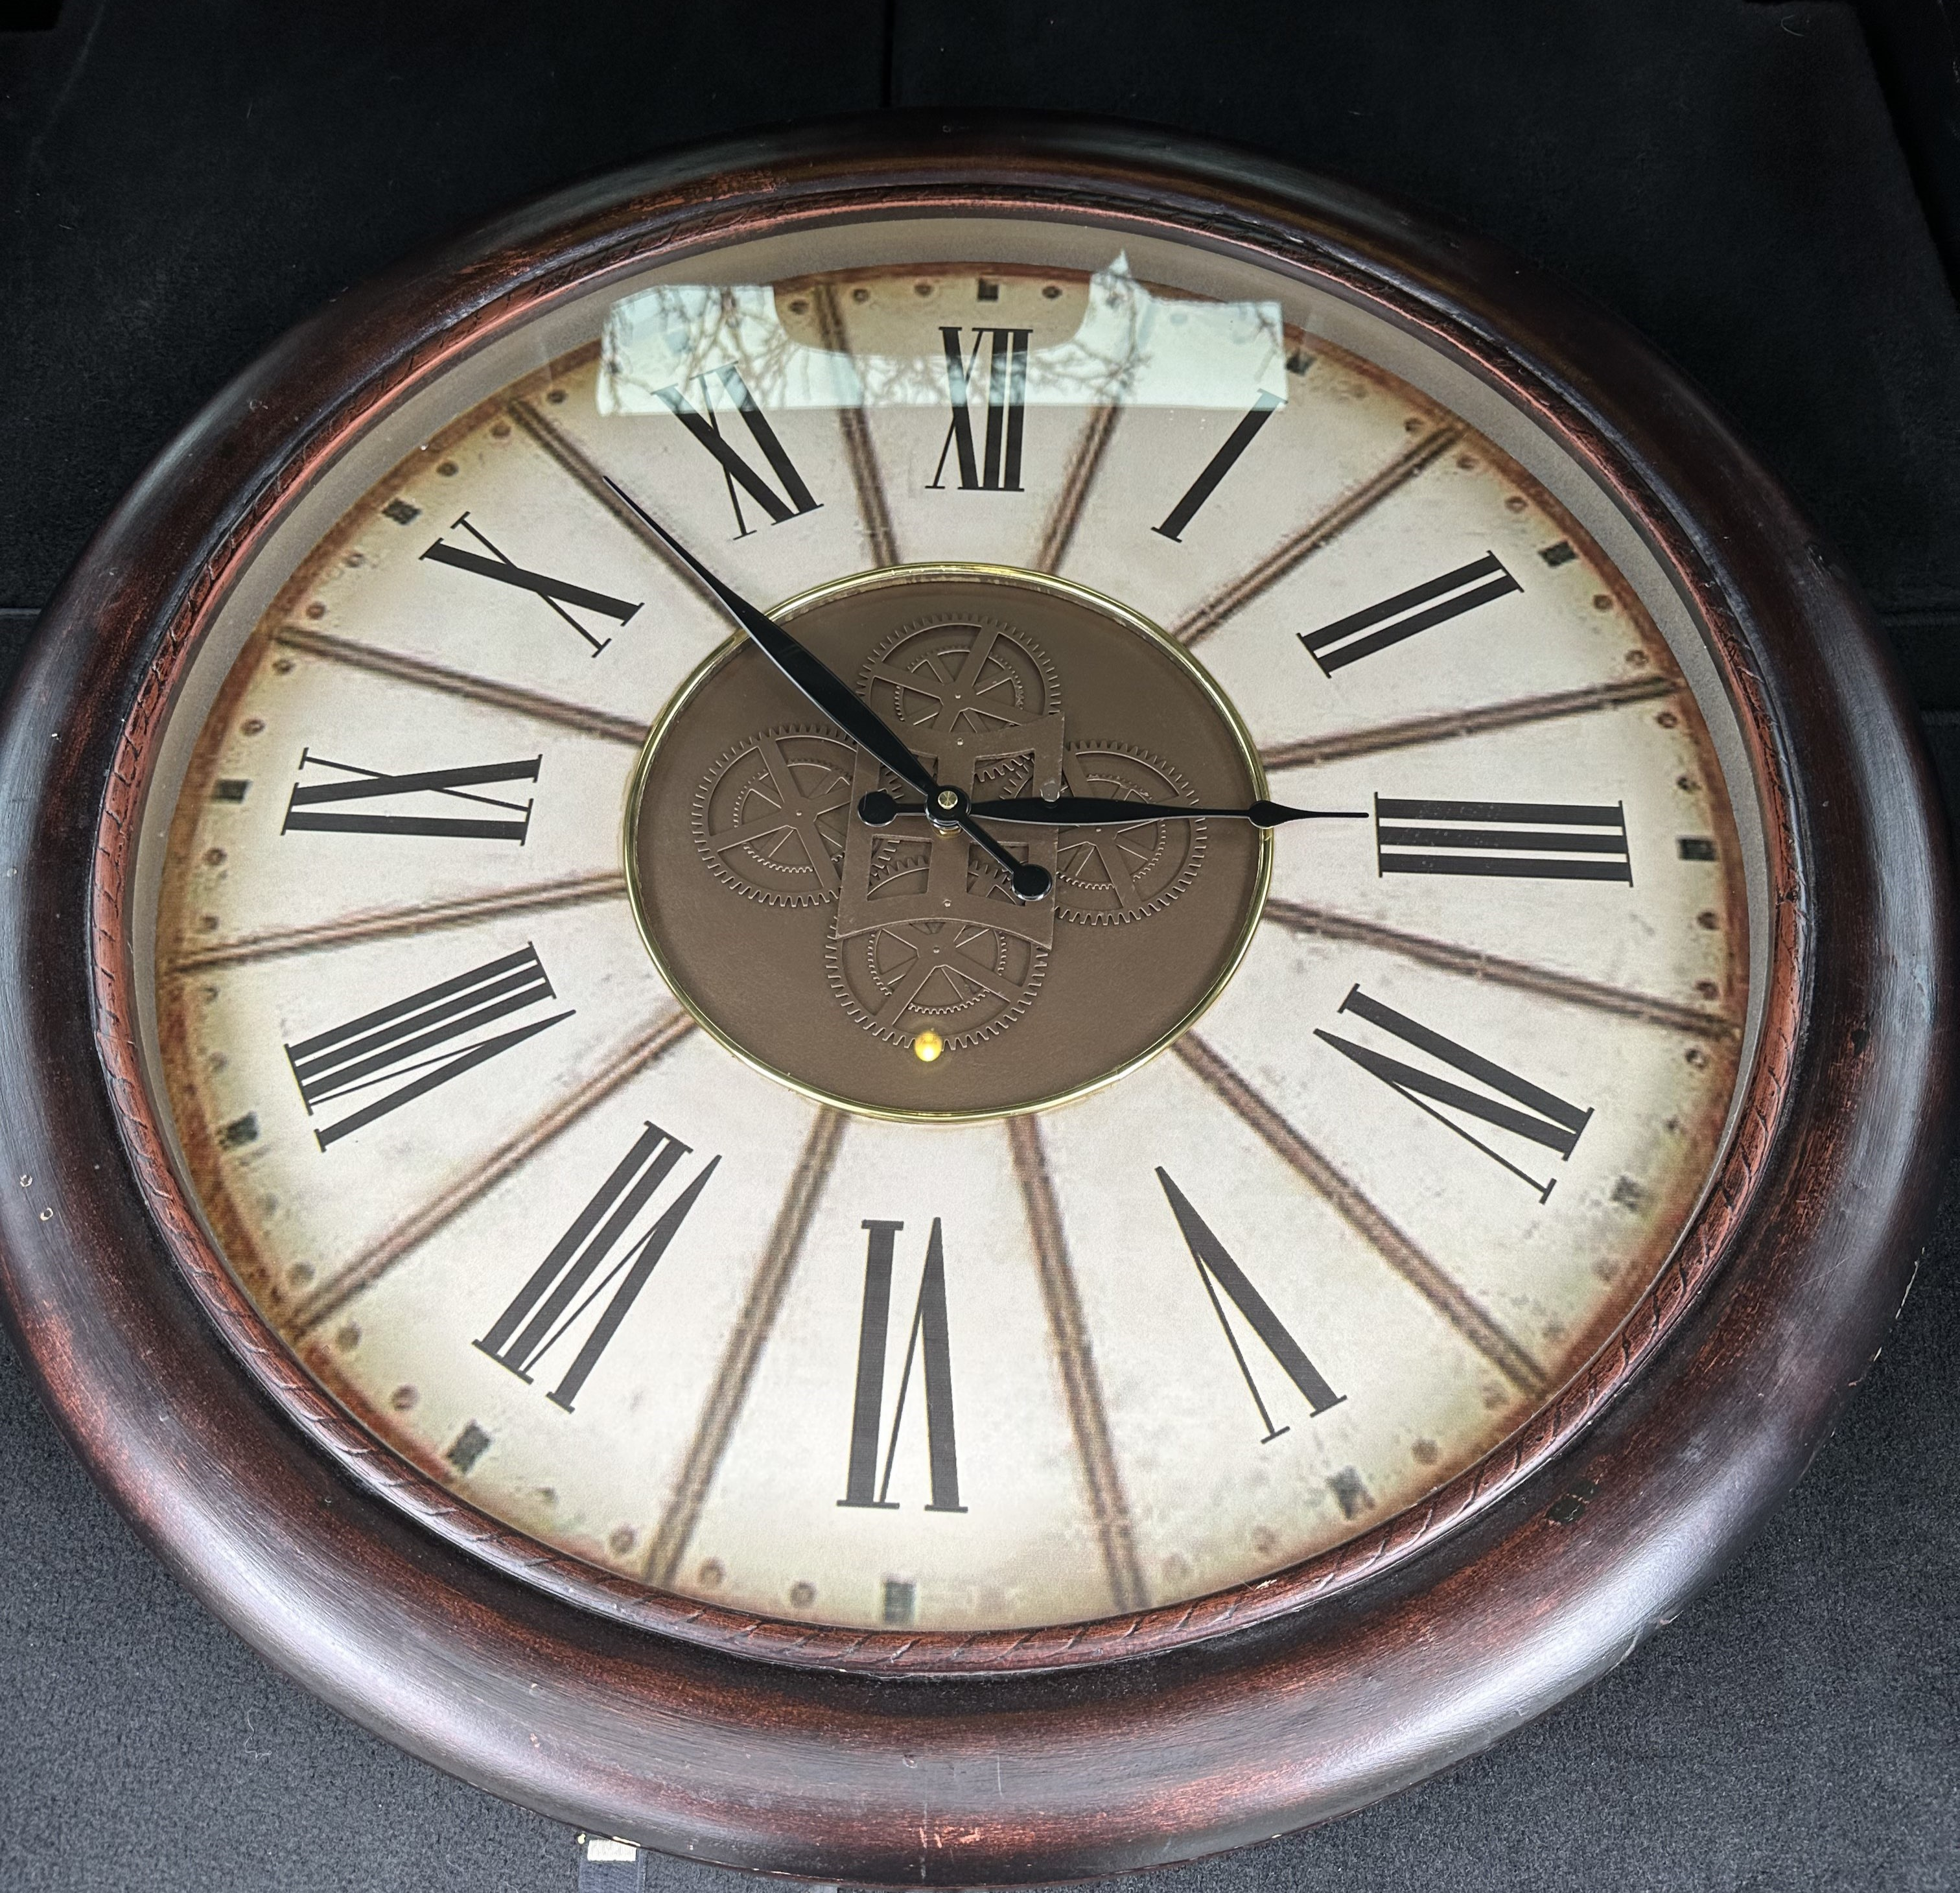
\includegraphics[width=0.85\columnwidth]{Images/big-clock.jpg}
    \caption{The big clock that we are using for the ``Player Clock''.}
\end{figure}

Our early prototype for this control is incredibly rough and does not use the microcontroller or the
motor that we are hoping to use in the final project, and is mostly just a proof of concept. In the
final project we are going to use a stepper motor that will allow us to have a much finer level of
control over what time the clock is displaying, and will also help the central computer keep track of
what time is being displayed. Furthermore, we are going to be 3D printing mounting brackets and other
components that will help the motor stay in place, rather than the mess of broken popsicle sticks and
duct tape that it currently is.

On top of the game clock is the game timer which will be displayed next to the door. This timer
shows the remaining amount of time left to complete the game and is visible at all times. When the
monster is revealed to the player during certain nighttime segments, the timer will go down at a
faster rate which will dissuade players from getting the monster's attention. Using an LED display,
the time will be outputted based on the value retrieved from the central computer's internal timer.



% *************************************************************************************************************************************
% ************************************* THIS SECTION MUST BE REVISED ******************************************************************
% *************************************************************************************************************************************
\section{Evaluation}


\begin{figure}[H]
    \centering
    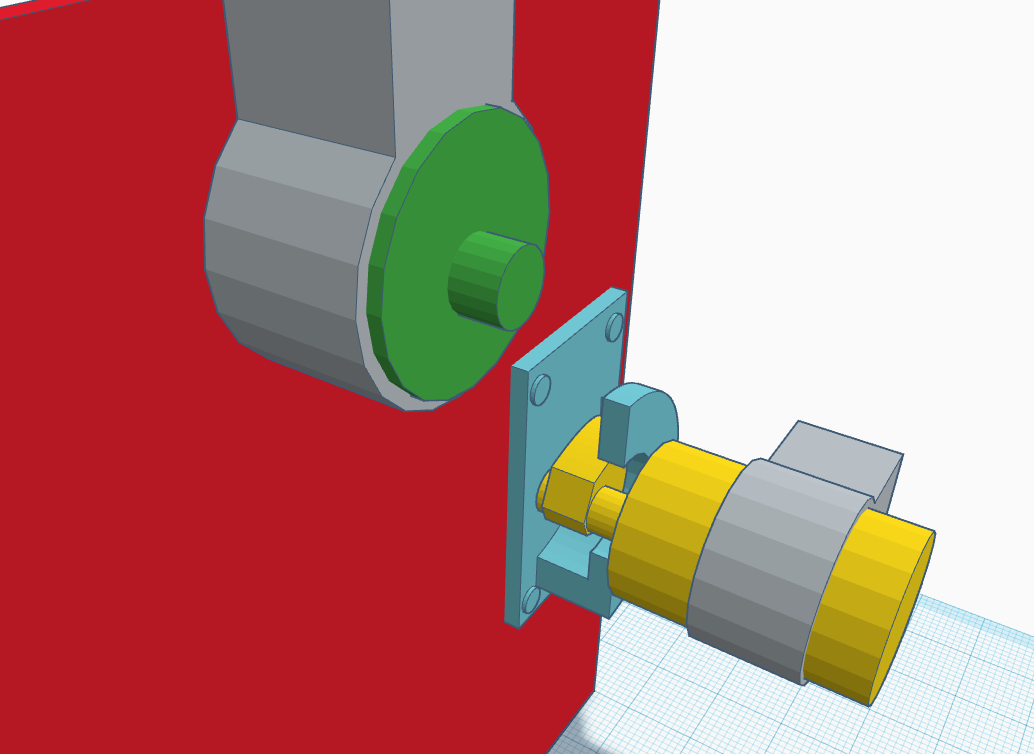
\includegraphics[width=0.85\columnwidth]{Images/ClosedLock.png}
    \caption{When the motor arms are under the metal plate, the container remains locked}
\end{figure}

\begin{figure}[H]
    \centering
    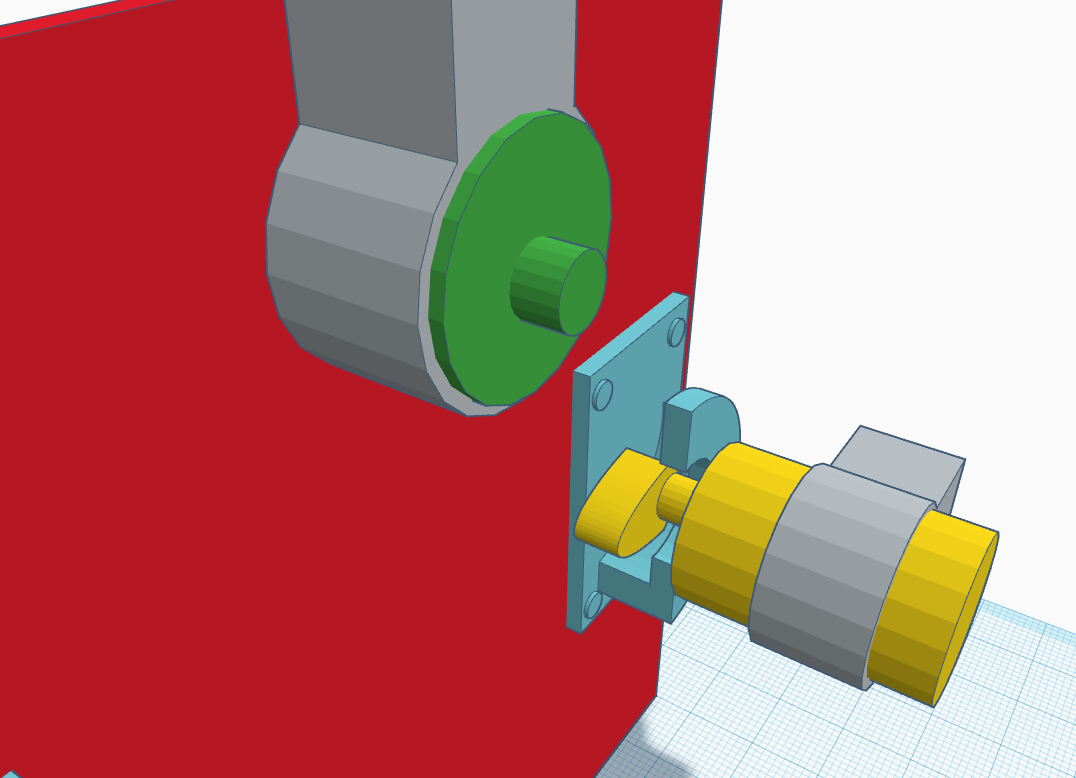
\includegraphics[width=0.85\columnwidth]{Images/OpenLock.png}
    \caption{When the arms are rotated out from the metal plate, the container is unlocked and can manually be opened.}
\end{figure}

\begin{figure}[H]
    \centering
    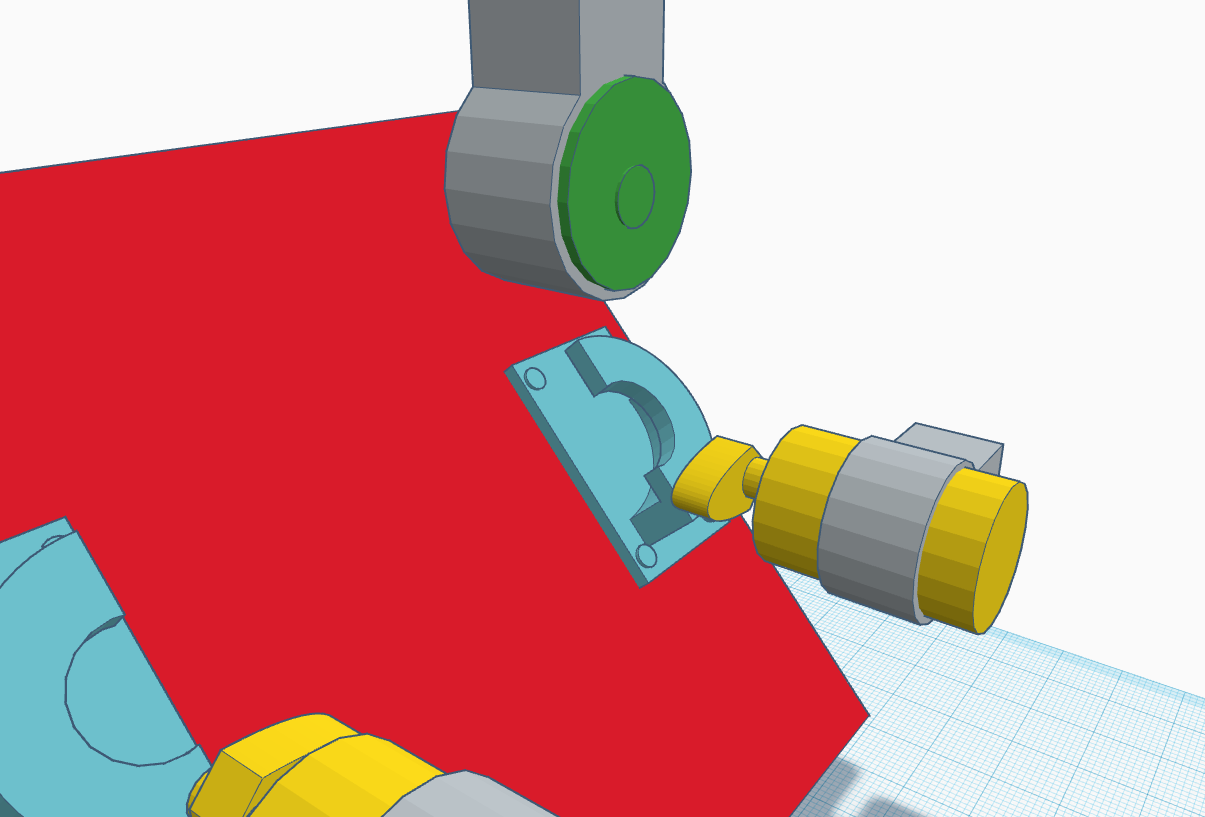
\includegraphics[width=0.85\columnwidth]{Images/OpenContainer.png}
    \caption{The internal solenoid can be used for several effects. For example, when facing the container opening, it can pop the
        door open automatically. If it is facing a wall, it will create a knock sound, or if it does not contact with anything, it can
        make a clicking noise to signal the box is unlocked.}
\end{figure}
 
% Probably want to keep this for the IMPLEMENTATION seciton above
\section{Communication Protocols}
As of now, we are trying to decide between two communication protocols that will be used
to control majority of the connections in our room. These two protocols are Wi-Fi and Zigbee,
and each of these have their unique benefits associated with them. A third communication
protocol, bluetooth, is also something that we are thinging of incorporating, however, this
will be more of a secondary communication protocol and will not be the driving force behind
how our components will communicate with each other.

\subsection*{Wi-Fi}
Wi-Fi will act as an incredibly reliable and secure option for our senior project. One of the benefits of Wi-Fi
is that is it so widely supported. There are lots of libraries that would make communication and connection over
Wi-Fi as simple as possible. Plus, the connection range is incredibly good over Wi-Fi, and the data rate is quite high
(around 54 Mbps)~\cite{wifiVsZigbee}. There are two drawbacks to Wi-Fi, however, the first being that it uses a bit more energy than Zigbee
to operate, which may become a problem depending on how many of our components need to operate on a portable energy
source. The second is that there are so many other devices that operate using Wi-Fi, and we may want the privacy that
a connection through Zigbee would provide.

\subsection*{Zigbee}
On the other hand, Zigbee would be an interesting option for a variety of reasons. The most beneficial reason to using
Zigbee would be its topology. Zigbee uses a mesh network topology, which allows each of the network devices to connect with
one another, rather than being dependent upon a central hub to manage the details of the escape room. This would decrease
the number of ``network-hops'' a command would need to traverse, allowing components to tell locks when their puzzle has been
solved. We may end up needing a central hub, so this benefit could nullified, but I digress. Furthermore, Zigbee is much less
widely used than Wi-Fi providing us with a unique experience when trying to get all of our components to communicate
with one another. It also consumes less energy and has a lower data transmission rate than Wi-Fi (maxing out at 250 Kbps),
which could help our wireless components be more energy efficient~\cite{wifiVsZigbee}. These details are yet to be explored,
however, and will need to be more properly considered when we have a more developed plan as to what our escape room is going to require.


%   ********************************************************************************************************
%   ********************* CONCLUSION TO BE COMPLETED TOGETHER **********************************************
%   ********************************************************************************************************
\section{Conclusions}
In conclusion, we are confident that this project will help us grow and become more capable
engineers in the future. We are going to learn more about how to deal with lots of interconnected
micro-systems, how to create a compelling and immersive story, how to properly document and track
our work, and how to work together as a team on a long-term development project. All of these things
are incredibly valuable to prospective employers, and we are excited to leave college as prepared
as possible to enter the workforce. Furthermore, this is a project that we are all incredibly excited
about, which will help us produce something that we can be proud of by the end of next semester!

\section{Appendix A: Reference Material}

\subsection{Bill of Materials}
In order to have a functioning project that we can be proud of, we are going to need a lot of materials.
A list of these materials have been included below
\begin{itemize}
    \item Programmable microcontrollers
    \item Analog clock
    \item Cameras
    \item Small CRT televisions
    \item Audio cassette player
    \item Writable audio cassette tapes
    \item MP3 digital audio controller
    \item Speakers
    \item Motors (To act as lock releases)
    \item Solenoids
    \item LED Display
    \item Adjustable RGB lights
    \item Wireless communication modules
    \item Storage containers
    \item Busts with detachable modules
\end{itemize}

\section{Appendix B: Troubles of note during development}

\begin{thebibliography}{00}

    \bibitem{wikipediaEscapeRoom} “Escape room,” Wikipedia, 10-Feb-2023. [Online]. Available: \url{https://en.wikipedia.org/wiki/Escape_room}. [Accessed: 24-Mar-2023].
    \bibitem{germanEscapeRoom} M. Pfeifer, B. Völker, S. Böttcher, S. Köhler, and P. M. Scholl, “Teaching embedded systems by constructing an escape room,” Proceedings of the 52nd ACM Technical Symposium on Computer Science Education, 2021.    
    \bibitem{whatIsAnEscapeRoom} A. Ascalon, “Escape rooms: Everything you need to know (2022),” Escape Rooms | Everything You Need To Know (2022), 01-Dec-2022. [Online]. Available:  \url{https://theescapegame.com/blog/what-is-an-escape-room/}. [Accessed: 24-Mar-2023].
    \bibitem{wifiVsZigbee} B. Priya, “What are the differences between Zigbee and Wi-Fi,” Tutorials Point, 17-Mar-2022. [Online]. Available: \url{https://www.tutorialspoint.com/what-are-the-differences-between-zigbee-and-wi-fi}. [Accessed: 03-May-2023].

\end{thebibliography}




\end{document}
